\section{The Schwarzschild Solution as Exterior Closure}
\label{sec:schwarzschild}

\subsection{What This Section Does}

Section~\ref{sec:einstein} showed that gravitational dynamics arise as a
fixed-point structure of closure density.
The next step is to examine the simplest configuration:
static, spherically symmetric, and with localized closure density.
\begin{equation}
  \boxed{\text{Closure concentrated at a single point.}}
\end{equation}
In general relativity, this leads to the Schwarzschild solution.
Within VED, the same structure emerges from modification of distance.

\subsection{Definition of the Exterior Vacuum}

Consider a localized closure distribution $L(x) = M\,\delta(x)$.
Outside the localized region ($r > R$), $L(r) = 0$.
In this region, closure density vanishes but the metric remains influenced
by the boundary conditions imposed by the central structure.

The potential equation becomes:
\begin{equation}
  \nabla^2\Psi \propto L = 0
  \qquad \Rightarrow \qquad
  \nabla^2\Psi = 0.
\end{equation}
For spherical symmetry, the solution is:
\begin{equation}
  \boxed{\Psi(r) = -\frac{G_{\text{eff}} M}{r}.}
\end{equation}
\begin{equation}
  \boxed{\text{The Newtonian potential.}}
\end{equation}

\subsection{Form of the Metric}

In the weak-gravity limit, the metric takes the form:
\begin{equation}
  \label{eq:schwarzschild_weak}
  \boxed{
    ds^2
    \approx
    -\!\left(1-\frac{2GM}{r}\right)dt^2
    +\left(1+\frac{2GM}{r}\right)dr^2
    + r^2 d\Omega^2.
  }
\end{equation}
This expression corresponds to the first-order expansion of the Schwarzschild metric.
\begin{equation}
  \boxed{\text{Consistent with the Schwarzschild solution (weak-gravity limit).}}
\end{equation}
The full nonlinear expression emerges when the fixed-point equation is solved
beyond linear order.

\subsection{What Is Happening}

General relativity interprets this solution as curvature of spacetime.
VED interprets it differently.
\begin{equation}
  \boxed{\text{Distance cost is modified by closure density.}}
\end{equation}
As a result, propagation paths change, light trajectories bend,
time dilation appears, and an effective metric emerges.
The observable consequences coincide, while the interpretation differs.

\subsection{VED Interpretation of the Horizon}

The Schwarzschild radius is $r_s = 2GM$.
At this radius, $g_{tt} \to 0$.
Within VED, this does not represent geometric breakdown.
\begin{equation}
  \boxed{\text{The horizon is a critical point of path structure.}}
\end{equation}
At this point, path cost diverges, propagation freezes,
and closure density approaches a critical value.
The horizon is therefore a phase boundary,
as illustrated in Figure~\ref{fig:phase_transition}.

\begin{figure}[h]
  \centering
  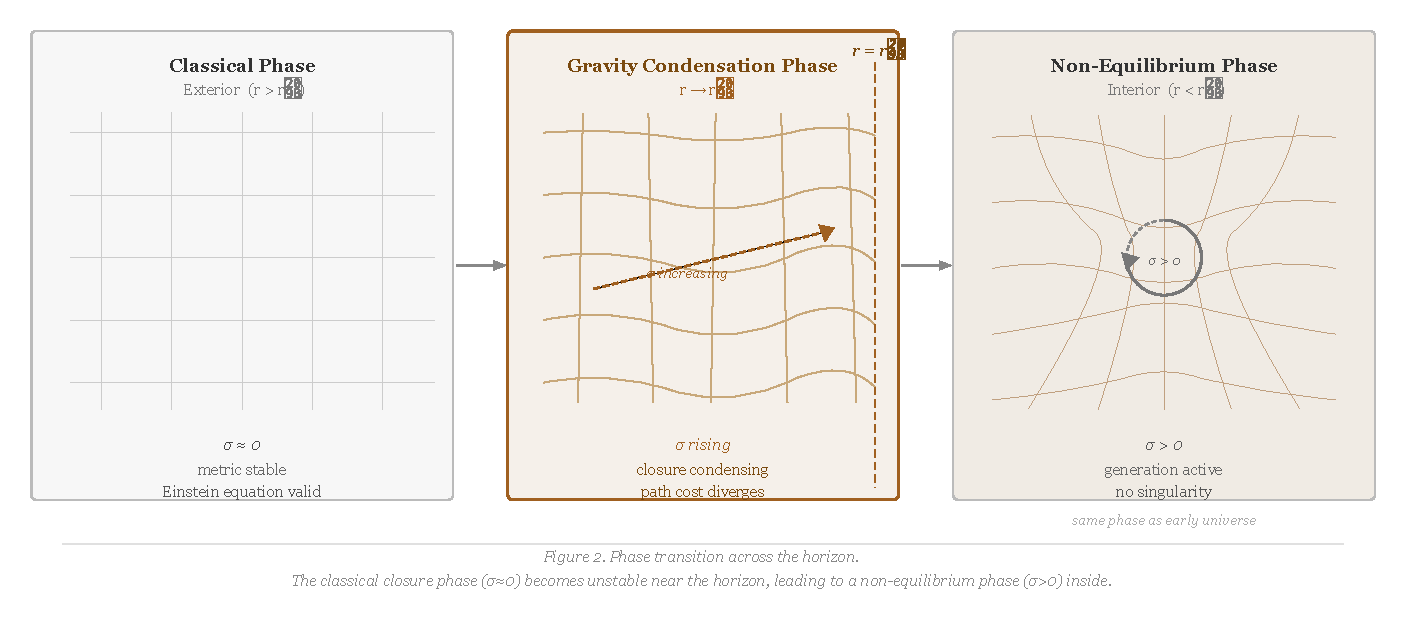
\includegraphics[width=\textwidth]{figures/VED_Vol3_Figure2.pdf}
  \caption{
    Phase transition across the horizon.
    The classical closure phase ($\sigma \approx 0$) becomes unstable
    near the horizon (gravity condensation phase),
    leading to a non-equilibrium phase ($\sigma > 0$) inside.
    The horizon corresponds to the transition region.
  }
  \label{fig:phase_transition}
\end{figure}

\subsection{Summary}

The exterior gravitational solution emerges naturally from closure density.
\begin{equation}
  \boxed{\text{The Schwarzschild solution appears as a limit of closure geometry.}}
\end{equation}
No new force or curvature postulate is required.
\begin{equation}
  \boxed{\text{Gravity emerges from modified distance.}}
\end{equation}
